\documentclass[twoside]{book}

% Packages required by doxygen
\usepackage{fixltx2e}
\usepackage{calc}
\usepackage{doxygen}
\usepackage{graphicx}
\usepackage[utf8]{inputenc}
\usepackage{makeidx}
\usepackage{multicol}
\usepackage{multirow}
\PassOptionsToPackage{warn}{textcomp}
\usepackage{textcomp}
\usepackage[nointegrals]{wasysym}
\usepackage[table]{xcolor}

% Font selection
\usepackage[T1]{fontenc}
\usepackage{mathptmx}
\usepackage[scaled=.90]{helvet}
\usepackage{courier}
\usepackage{amssymb}
\usepackage{sectsty}
\renewcommand{\familydefault}{\sfdefault}
\allsectionsfont{%
  \fontseries{bc}\selectfont%
  \color{darkgray}%
}
\renewcommand{\DoxyLabelFont}{%
  \fontseries{bc}\selectfont%
  \color{darkgray}%
}
\newcommand{\+}{\discretionary{\mbox{\scriptsize$\hookleftarrow$}}{}{}}

% Page & text layout
\usepackage{geometry}
\geometry{%
  a4paper,%
  top=2.5cm,%
  bottom=2.5cm,%
  left=2.5cm,%
  right=2.5cm%
}
\tolerance=750
\hfuzz=15pt
\hbadness=750
\setlength{\emergencystretch}{15pt}
\setlength{\parindent}{0cm}
\setlength{\parskip}{0.2cm}
\makeatletter
\renewcommand{\paragraph}{%
  \@startsection{paragraph}{4}{0ex}{-1.0ex}{1.0ex}{%
    \normalfont\normalsize\bfseries\SS@parafont%
  }%
}
\renewcommand{\subparagraph}{%
  \@startsection{subparagraph}{5}{0ex}{-1.0ex}{1.0ex}{%
    \normalfont\normalsize\bfseries\SS@subparafont%
  }%
}
\makeatother

% Headers & footers
\usepackage{fancyhdr}
\pagestyle{fancyplain}
\fancyhead[LE]{\fancyplain{}{\bfseries\thepage}}
\fancyhead[CE]{\fancyplain{}{}}
\fancyhead[RE]{\fancyplain{}{\bfseries\leftmark}}
\fancyhead[LO]{\fancyplain{}{\bfseries\rightmark}}
\fancyhead[CO]{\fancyplain{}{}}
\fancyhead[RO]{\fancyplain{}{\bfseries\thepage}}
\fancyfoot[LE]{\fancyplain{}{}}
\fancyfoot[CE]{\fancyplain{}{}}
\fancyfoot[RE]{\fancyplain{}{\bfseries\scriptsize Generated on Mon Oct 13 2014 11\+:05\+:25 for My Project by Doxygen }}
\fancyfoot[LO]{\fancyplain{}{\bfseries\scriptsize Generated on Mon Oct 13 2014 11\+:05\+:25 for My Project by Doxygen }}
\fancyfoot[CO]{\fancyplain{}{}}
\fancyfoot[RO]{\fancyplain{}{}}
\renewcommand{\footrulewidth}{0.4pt}
\renewcommand{\chaptermark}[1]{%
  \markboth{#1}{}%
}
\renewcommand{\sectionmark}[1]{%
  \markright{\thesection\ #1}%
}

% Indices & bibliography
\usepackage{natbib}
\usepackage[titles]{tocloft}
\setcounter{tocdepth}{3}
\setcounter{secnumdepth}{5}
\makeindex

% Hyperlinks (required, but should be loaded last)
\usepackage{ifpdf}
\ifpdf
  \usepackage[pdftex,pagebackref=true]{hyperref}
\else
  \usepackage[ps2pdf,pagebackref=true]{hyperref}
\fi
\hypersetup{%
  colorlinks=true,%
  linkcolor=blue,%
  citecolor=blue,%
  unicode%
}

% Custom commands
\newcommand{\clearemptydoublepage}{%
  \newpage{\pagestyle{empty}\cleardoublepage}%
}


%===== C O N T E N T S =====

\begin{document}

% Titlepage & ToC
\hypersetup{pageanchor=false,
             bookmarks=true,
             bookmarksnumbered=true,
             pdfencoding=unicode
            }
\pagenumbering{roman}
\begin{titlepage}
\vspace*{7cm}
\begin{center}%
{\Large My Project }\\
\vspace*{1cm}
{\large Generated by Doxygen 1.8.8}\\
\vspace*{0.5cm}
{\small Mon Oct 13 2014 11:05:25}\\
\end{center}
\end{titlepage}
\clearemptydoublepage
\tableofcontents
\clearemptydoublepage
\pagenumbering{arabic}
\hypersetup{pageanchor=true}

%--- Begin generated contents ---
\chapter{Todo List}
\label{todo}
\hypertarget{todo}{}

\begin{DoxyRefList}
\item[\label{todo__todo000001}%
\hypertarget{todo__todo000001}{}%
File \hyperlink{ConfigRegs18f4520_8h}{Config\+Regs18f4520.h} ]Consider if Watchdog Timer should be enabled for production code, and add W\+D\+T management code if so.

Consider if Stack Overflow Reset should be enabled for production code. It may be better not to, as there is no re-\/entrant or recursive code, or dynamic memory allocation here -\/ if the code loads statically it should run.

Change startup code c016iz.\+c so that everything (including initialised variables) correctly re-\/starts if \hyperlink{HardUItest_8c_a6288eba0f8e8ad3ab1544ad731eb7667}{main()} ever exits or a B\+O\+R or W\+D\+T reset occurs.  
\item[\label{todo__todo000004}%
\hypertarget{todo__todo000004}{}%
Global \hyperlink{LCD_8c_a6d7066138d22070be0234d8b113cf776}{delay} (unsigned int t)]Complete, test, debug and document this code!!! 
\item[\label{todo__todo000005}%
\hypertarget{todo__todo000005}{}%
Global \hyperlink{Range_8h_aff3698f3a7b3b5963d8e6b305a165d71}{range} (void)]Read in temperature for U\+S calculation  
\item[\label{todo__todo000006}%
\hypertarget{todo__todo000006}{}%
Global \hyperlink{Temp_8h_a4946ccbc1990e831667bffded1147c4f}{read\+Tempx2} (void)]Test and debug this function 
\end{DoxyRefList}
\chapter{Class Index}
\section{Data Structures}
Here are the data structures with brief descriptions\+:\begin{DoxyCompactList}
\item\contentsline{section}{\hyperlink{structcircularBuffer}{circular\+Buffer} \\*Stores bytes of data in a circular buffer }{\pageref{structcircularBuffer}}{}
\item\contentsline{section}{\hyperlink{structDelay}{Delay} }{\pageref{structDelay}}{}
\item\contentsline{section}{\hyperlink{structDirection}{Direction} \\*Stores an inclination and azimuth }{\pageref{structDirection}}{}
\item\contentsline{section}{\hyperlink{structSubMenu}{Sub\+Menu} }{\pageref{structSubMenu}}{}
\item\contentsline{section}{\hyperlink{structsystemState}{system\+State} \\*Stores the current state of the system }{\pageref{structsystemState}}{}
\item\contentsline{section}{\hyperlink{structTrackingData}{Tracking\+Data} \\*Stores the current target information }{\pageref{structTrackingData}}{}
\end{DoxyCompactList}

\chapter{File Index}
\section{File List}
Here is a list of all files with brief descriptions\+:\begin{DoxyCompactList}
\item\contentsline{section}{Yavin4\+Defence\+System/\+Code/\hyperlink{CircularBuffers_8h}{Circular\+Buffers.\+h} }{\pageref{CircularBuffers_8h}}{}
\item\contentsline{section}{Yavin4\+Defence\+System/\+Code/\hyperlink{Common_8h}{Common.\+h} }{\pageref{Common_8h}}{}
\item\contentsline{section}{Yavin4\+Defence\+System/\+Code/\hyperlink{ConfigRegs18f4520_8h}{Config\+Regs18f4520.\+h} \\*Include file to set the Configuration Bits of a P\+I\+C18\+F4520 }{\pageref{ConfigRegs18f4520_8h}}{}
\item\contentsline{section}{Yavin4\+Defence\+System/\+Code/\hyperlink{EEPROM_8c}{E\+E\+P\+R\+O\+M.\+c} }{\pageref{EEPROM_8c}}{}
\item\contentsline{section}{Yavin4\+Defence\+System/\+Code/\hyperlink{HardUItest_8c}{Hard\+U\+Itest.\+c} }{\pageref{HardUItest_8c}}{}
\item\contentsline{section}{Yavin4\+Defence\+System/\+Code/\hyperlink{HardUItest_8h}{Hard\+U\+Itest.\+h} }{\pageref{HardUItest_8h}}{}
\item\contentsline{section}{Yavin4\+Defence\+System/\+Code/\hyperlink{Interrupts_8c}{Interrupts.\+c} }{\pageref{Interrupts_8c}}{}
\item\contentsline{section}{Yavin4\+Defence\+System/\+Code/\hyperlink{LCD_8c}{L\+C\+D.\+c} }{\pageref{LCD_8c}}{}
\item\contentsline{section}{Yavin4\+Defence\+System/\+Code/\hyperlink{LCD_8h}{L\+C\+D.\+h} }{\pageref{LCD_8h}}{}
\item\contentsline{section}{Yavin4\+Defence\+System/\+Code/\hyperlink{LCD__defs_8h}{L\+C\+D\+\_\+defs.\+h} }{\pageref{LCD__defs_8h}}{}
\item\contentsline{section}{Yavin4\+Defence\+System/\+Code/\hyperlink{MenuDefs_8h}{Menu\+Defs.\+h} }{\pageref{MenuDefs_8h}}{}
\item\contentsline{section}{Yavin4\+Defence\+System/\+Code/\hyperlink{Menusystem_8c}{Menusystem.\+c} }{\pageref{Menusystem_8c}}{}
\item\contentsline{section}{Yavin4\+Defence\+System/\+Code/\hyperlink{Menusystem_8h}{Menusystem.\+h} }{\pageref{Menusystem_8h}}{}
\item\contentsline{section}{Yavin4\+Defence\+System/\+Code/\hyperlink{Menusystem2_8c}{Menusystem2.\+c} }{\pageref{Menusystem2_8c}}{}
\item\contentsline{section}{Yavin4\+Defence\+System/\+Code/\hyperlink{newfile_8h}{newfile.\+h} }{\pageref{newfile_8h}}{}
\item\contentsline{section}{Yavin4\+Defence\+System/\+Code/\hyperlink{newmain_8c}{newmain.\+c} }{\pageref{newmain_8c}}{}
\item\contentsline{section}{Yavin4\+Defence\+System/\+Code/\hyperlink{p18f4520_8h}{p18f4520.\+h} }{\pageref{p18f4520_8h}}{}
\item\contentsline{section}{Yavin4\+Defence\+System/\+Code/\hyperlink{PanTilt_8c}{Pan\+Tilt.\+c} }{\pageref{PanTilt_8c}}{}
\item\contentsline{section}{Yavin4\+Defence\+System/\+Code/\hyperlink{PanTilt_8h}{Pan\+Tilt.\+h} }{\pageref{PanTilt_8h}}{}
\item\contentsline{section}{Yavin4\+Defence\+System/\+Code/\hyperlink{Range_8c}{Range.\+c} }{\pageref{Range_8c}}{}
\item\contentsline{section}{Yavin4\+Defence\+System/\+Code/\hyperlink{Range_8h}{Range.\+h} }{\pageref{Range_8h}}{}
\item\contentsline{section}{Yavin4\+Defence\+System/\+Code/\hyperlink{ROM2RAM_8c}{R\+O\+M2\+R\+A\+M.\+c} }{\pageref{ROM2RAM_8c}}{}
\item\contentsline{section}{Yavin4\+Defence\+System/\+Code/\hyperlink{Serial_8c}{Serial.\+c} }{\pageref{Serial_8c}}{}
\item\contentsline{section}{Yavin4\+Defence\+System/\+Code/\hyperlink{Serial_8h}{Serial.\+h} }{\pageref{Serial_8h}}{}
\item\contentsline{section}{Yavin4\+Defence\+System/\+Code/\hyperlink{Temp_8c}{Temp.\+c} }{\pageref{Temp_8c}}{}
\item\contentsline{section}{Yavin4\+Defence\+System/\+Code/\hyperlink{Temp_8h}{Temp.\+h} }{\pageref{Temp_8h}}{}
\item\contentsline{section}{Yavin4\+Defence\+System/\+Code/\hyperlink{Tracking_8c}{Tracking.\+c} }{\pageref{Tracking_8c}}{}
\item\contentsline{section}{Yavin4\+Defence\+System/\+Code/\hyperlink{Tracking_8h}{Tracking.\+h} }{\pageref{Tracking_8h}}{}
\item\contentsline{section}{Yavin4\+Defence\+System/\+Code/\hyperlink{usart_8h}{usart.\+h} }{\pageref{usart_8h}}{}
\item\contentsline{section}{Yavin4\+Defence\+System/\+Code/\hyperlink{User__Interface_8c}{User\+\_\+\+Interface.\+c} }{\pageref{User__Interface_8c}}{}
\item\contentsline{section}{Yavin4\+Defence\+System/\+Code/\hyperlink{User__Interface_8h}{User\+\_\+\+Interface.\+h} }{\pageref{User__Interface_8h}}{}
\end{DoxyCompactList}

\chapter{Class Documentation}
\hypertarget{structcircular_buffer}{\section{circular\+Buffer Struct Reference}
\label{structcircular_buffer}\index{circular\+Buffer@{circular\+Buffer}}
}


Stores bytes of data in a circular buffer.  




{\ttfamily \#include $<$Circular\+Buffers.\+h$>$}

\subsection*{Data Fields}
\begin{DoxyCompactItemize}
\item 
unsigned char \hyperlink{structcircular_buffer_a47f7e6109597e5c1c227993c0ce5f560}{head}
\item 
unsigned char \hyperlink{structcircular_buffer_af18a1d7542e277284c4794593b049258}{tail}
\item 
unsigned char \hyperlink{structcircular_buffer_ad7b57ba90694482456be1fbab7de4aec}{data} \mbox{[}\hyperlink{_circular_buffers_8h_a5a69f707d5405fe875b322c6bfbace46}{B\+U\+F\+F\+E\+R\+L\+E\+N\+G\+T\+H}\mbox{]}
\end{DoxyCompactItemize}


\subsection{Detailed Description}
Stores bytes of data in a circular buffer. 



 typedef of \hyperlink{structcircular_buffer}{circular\+Buffer} struct

Length\+: B\+U\+F\+F\+E\+R\+L\+E\+N\+G\+T\+H

Description\+: Defines a circular buffer in which bytes of data can be placed, or removed at any time in the correct order that they were pushed. The accompanying functionality facilitates all necessary circular buffer related operations. This implementation reduces the buffer length by 1 to differentiate between full and empty states. B\+U\+F\+F\+E\+R\+L\+E\+N\+G\+T\+H can be redefined in individual files to get different buffer lengths 

Definition at line 49 of file Circular\+Buffers.\+h.



\subsection{Field Documentation}
\hypertarget{structcircular_buffer_ad7b57ba90694482456be1fbab7de4aec}{\index{circular\+Buffer@{circular\+Buffer}!data@{data}}
\index{data@{data}!circular\+Buffer@{circular\+Buffer}}
\subsubsection[{data}]{\setlength{\rightskip}{0pt plus 5cm}unsigned char data\mbox{[}{\bf B\+U\+F\+F\+E\+R\+L\+E\+N\+G\+T\+H}\mbox{]}}}\label{structcircular_buffer_ad7b57ba90694482456be1fbab7de4aec}


Definition at line 53 of file Circular\+Buffers.\+h.

\hypertarget{structcircular_buffer_a47f7e6109597e5c1c227993c0ce5f560}{\index{circular\+Buffer@{circular\+Buffer}!head@{head}}
\index{head@{head}!circular\+Buffer@{circular\+Buffer}}
\subsubsection[{head}]{\setlength{\rightskip}{0pt plus 5cm}unsigned char head}}\label{structcircular_buffer_a47f7e6109597e5c1c227993c0ce5f560}


Definition at line 51 of file Circular\+Buffers.\+h.

\hypertarget{structcircular_buffer_af18a1d7542e277284c4794593b049258}{\index{circular\+Buffer@{circular\+Buffer}!tail@{tail}}
\index{tail@{tail}!circular\+Buffer@{circular\+Buffer}}
\subsubsection[{tail}]{\setlength{\rightskip}{0pt plus 5cm}unsigned char tail}}\label{structcircular_buffer_af18a1d7542e277284c4794593b049258}


Definition at line 52 of file Circular\+Buffers.\+h.



The documentation for this struct was generated from the following file\+:\begin{DoxyCompactItemize}
\item 
\hyperlink{_circular_buffers_8h}{Circular\+Buffers.\+h}\end{DoxyCompactItemize}

\hypertarget{struct_delay}{\section{Delay Struct Reference}
\label{struct_delay}\index{Delay@{Delay}}
}
\subsection*{Public Attributes}
\begin{DoxyCompactItemize}
\item 
\hypertarget{struct_delay_a4cb4f750cd566d1a1cf61d1fa93d5ce3}{signed int {\bfseries Azimuth\+Delay}}\label{struct_delay_a4cb4f750cd566d1a1cf61d1fa93d5ce3}

\item 
\hypertarget{struct_delay_a19ac2a6a70e80fc14128af5716580d12}{signed int {\bfseries Inclination\+Delay}}\label{struct_delay_a19ac2a6a70e80fc14128af5716580d12}

\end{DoxyCompactItemize}


The documentation for this struct was generated from the following file\+:\begin{DoxyCompactItemize}
\item 
Pan\+Tilt.\+c\end{DoxyCompactItemize}

\hypertarget{struct_direction}{\section{Direction Struct Reference}
\label{struct_direction}\index{Direction@{Direction}}
}


Stores an inclination and azimuth.  




{\ttfamily \#include $<$Common.\+h$>$}

\subsection*{Data Fields}
\begin{DoxyCompactItemize}
\item 
int \hyperlink{struct_direction_a866e78e12cb32dcaf1ded89bda8be8f5}{azimuth}
\item 
int \hyperlink{struct_direction_af308b9934394c8bcf7614eb1df2d863f}{inclination}
\end{DoxyCompactItemize}


\subsection{Detailed Description}
Stores an inclination and azimuth. 



 typedef of \hyperlink{struct_direction}{Direction} struct

Description\+: A fully defined direction in which to point the pan tilt actuator or any other such purpose

Elements\+: -\/\+Azimuth\+: Contains the azimuth component of the direction (generally degrees) -\/\+Inclination\+: Contains the inclination component of the direction (generally degrees) 

Definition at line 70 of file Common.\+h.



\subsection{Field Documentation}
\hypertarget{struct_direction_a866e78e12cb32dcaf1ded89bda8be8f5}{\index{Direction@{Direction}!azimuth@{azimuth}}
\index{azimuth@{azimuth}!Direction@{Direction}}
\subsubsection[{azimuth}]{\setlength{\rightskip}{0pt plus 5cm}int azimuth}}\label{struct_direction_a866e78e12cb32dcaf1ded89bda8be8f5}


Definition at line 72 of file Common.\+h.

\hypertarget{struct_direction_af308b9934394c8bcf7614eb1df2d863f}{\index{Direction@{Direction}!inclination@{inclination}}
\index{inclination@{inclination}!Direction@{Direction}}
\subsubsection[{inclination}]{\setlength{\rightskip}{0pt plus 5cm}int inclination}}\label{struct_direction_af308b9934394c8bcf7614eb1df2d863f}


Definition at line 73 of file Common.\+h.



The documentation for this struct was generated from the following file\+:\begin{DoxyCompactItemize}
\item 
\hyperlink{_common_8h}{Common.\+h}\end{DoxyCompactItemize}

\hypertarget{struct_direction_state}{\section{Direction\+State Struct Reference}
\label{struct_direction_state}\index{Direction\+State@{Direction\+State}}
}
\subsection*{Public Attributes}
\begin{DoxyCompactItemize}
\item 
\hypertarget{struct_direction_state_a50d85e1e692dc39dcf03754cb1154d42}{int {\bfseries azimuth}}\label{struct_direction_state_a50d85e1e692dc39dcf03754cb1154d42}

\item 
\hypertarget{struct_direction_state_a3a2380ada725f632f657484da6d7627e}{int {\bfseries inclination}}\label{struct_direction_state_a3a2380ada725f632f657484da6d7627e}

\end{DoxyCompactItemize}


The documentation for this struct was generated from the following file\+:\begin{DoxyCompactItemize}
\item 
Common.\+h\end{DoxyCompactItemize}

\hypertarget{struct_sub_menu}{\section{Sub\+Menu Struct Reference}
\label{struct_sub_menu}\index{Sub\+Menu@{Sub\+Menu}}
}


Collaboration diagram for Sub\+Menu\+:\nopagebreak
\begin{figure}[H]
\begin{center}
\leavevmode
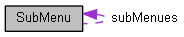
\includegraphics[width=210pt]{struct_sub_menu__coll__graph}
\end{center}
\end{figure}
\subsection*{Data Fields}
\begin{DoxyCompactItemize}
\item 
char \hyperlink{struct_sub_menu_a24706f7b55951b0e21967a256e107936}{serial\+Message} \mbox{[}\hyperlink{_menusystem2_8c_af3a7cb33a5ae7392934b3197ac67e080}{M\+A\+X\+\_\+\+S\+E\+R\+\_\+\+M\+S\+G\+\_\+\+L\+E\+N}\mbox{]}
\item 
char \hyperlink{struct_sub_menu_a10ce8be3d2bbadbc9c262b6be4bb3aec}{lcd\+Message} \mbox{[}\hyperlink{_menusystem2_8c_a803e4f9d2e28d9ab24055cb970ea12c3}{M\+A\+X\+\_\+\+L\+C\+D\+\_\+\+M\+S\+G\+\_\+\+L\+E\+N}\mbox{]}
\item 
char \hyperlink{struct_sub_menu_adcfcbb5b5340baf34c70fb8f4cc66f72}{serial\+Options} \mbox{[}\hyperlink{_menusystem2_8c_ab86e62ee54aa604cfbdc4d3048c2845d}{M\+A\+X\+\_\+\+N\+U\+M\+\_\+\+O\+P\+T\+I\+O\+N\+S}\mbox{]}
\item 
char \hyperlink{struct_sub_menu_aef0980fb751ef312c4ff945539aa3cd4}{inpt\+Options} \mbox{[}\hyperlink{_menusystem2_8c_ab86e62ee54aa604cfbdc4d3048c2845d}{M\+A\+X\+\_\+\+N\+U\+M\+\_\+\+O\+P\+T\+I\+O\+N\+S}\mbox{]}
\item 
void($\ast$ \hyperlink{struct_sub_menu_a1dae2f8dad8e2d2a30b13ee69ea542db}{numeric\+Function} )(int)
\item 
void($\ast$ \hyperlink{struct_sub_menu_ad86a4714605654261200ef4194e1657c}{default\+Function} )(void)
\item 
struct \hyperlink{struct_sub_menu}{Sub\+Menu} $\ast$ \hyperlink{struct_sub_menu_a915aa121e09e4c3f914dc59727f390e3}{sub\+Menues}
\end{DoxyCompactItemize}


\subsection{Detailed Description}


Definition at line 11 of file Menusystem2.\+c.



\subsection{Field Documentation}
\hypertarget{struct_sub_menu_ad86a4714605654261200ef4194e1657c}{\index{Sub\+Menu@{Sub\+Menu}!default\+Function@{default\+Function}}
\index{default\+Function@{default\+Function}!Sub\+Menu@{Sub\+Menu}}
\subsubsection[{default\+Function}]{\setlength{\rightskip}{0pt plus 5cm}void($\ast$ default\+Function)(void)}}\label{struct_sub_menu_ad86a4714605654261200ef4194e1657c}


Definition at line 19 of file Menusystem2.\+c.

\hypertarget{struct_sub_menu_aef0980fb751ef312c4ff945539aa3cd4}{\index{Sub\+Menu@{Sub\+Menu}!inpt\+Options@{inpt\+Options}}
\index{inpt\+Options@{inpt\+Options}!Sub\+Menu@{Sub\+Menu}}
\subsubsection[{inpt\+Options}]{\setlength{\rightskip}{0pt plus 5cm}char inpt\+Options\mbox{[}{\bf M\+A\+X\+\_\+\+N\+U\+M\+\_\+\+O\+P\+T\+I\+O\+N\+S}\mbox{]}}}\label{struct_sub_menu_aef0980fb751ef312c4ff945539aa3cd4}


Definition at line 16 of file Menusystem2.\+c.

\hypertarget{struct_sub_menu_a10ce8be3d2bbadbc9c262b6be4bb3aec}{\index{Sub\+Menu@{Sub\+Menu}!lcd\+Message@{lcd\+Message}}
\index{lcd\+Message@{lcd\+Message}!Sub\+Menu@{Sub\+Menu}}
\subsubsection[{lcd\+Message}]{\setlength{\rightskip}{0pt plus 5cm}char lcd\+Message\mbox{[}{\bf M\+A\+X\+\_\+\+L\+C\+D\+\_\+\+M\+S\+G\+\_\+\+L\+E\+N}\mbox{]}}}\label{struct_sub_menu_a10ce8be3d2bbadbc9c262b6be4bb3aec}


Definition at line 14 of file Menusystem2.\+c.

\hypertarget{struct_sub_menu_a1dae2f8dad8e2d2a30b13ee69ea542db}{\index{Sub\+Menu@{Sub\+Menu}!numeric\+Function@{numeric\+Function}}
\index{numeric\+Function@{numeric\+Function}!Sub\+Menu@{Sub\+Menu}}
\subsubsection[{numeric\+Function}]{\setlength{\rightskip}{0pt plus 5cm}void($\ast$ numeric\+Function)(int)}}\label{struct_sub_menu_a1dae2f8dad8e2d2a30b13ee69ea542db}


Definition at line 18 of file Menusystem2.\+c.

\hypertarget{struct_sub_menu_a24706f7b55951b0e21967a256e107936}{\index{Sub\+Menu@{Sub\+Menu}!serial\+Message@{serial\+Message}}
\index{serial\+Message@{serial\+Message}!Sub\+Menu@{Sub\+Menu}}
\subsubsection[{serial\+Message}]{\setlength{\rightskip}{0pt plus 5cm}char serial\+Message\mbox{[}{\bf M\+A\+X\+\_\+\+S\+E\+R\+\_\+\+M\+S\+G\+\_\+\+L\+E\+N}\mbox{]}}}\label{struct_sub_menu_a24706f7b55951b0e21967a256e107936}


Definition at line 13 of file Menusystem2.\+c.

\hypertarget{struct_sub_menu_adcfcbb5b5340baf34c70fb8f4cc66f72}{\index{Sub\+Menu@{Sub\+Menu}!serial\+Options@{serial\+Options}}
\index{serial\+Options@{serial\+Options}!Sub\+Menu@{Sub\+Menu}}
\subsubsection[{serial\+Options}]{\setlength{\rightskip}{0pt plus 5cm}char serial\+Options\mbox{[}{\bf M\+A\+X\+\_\+\+N\+U\+M\+\_\+\+O\+P\+T\+I\+O\+N\+S}\mbox{]}}}\label{struct_sub_menu_adcfcbb5b5340baf34c70fb8f4cc66f72}


Definition at line 15 of file Menusystem2.\+c.

\hypertarget{struct_sub_menu_a915aa121e09e4c3f914dc59727f390e3}{\index{Sub\+Menu@{Sub\+Menu}!sub\+Menues@{sub\+Menues}}
\index{sub\+Menues@{sub\+Menues}!Sub\+Menu@{Sub\+Menu}}
\subsubsection[{sub\+Menues}]{\setlength{\rightskip}{0pt plus 5cm}struct {\bf Sub\+Menu}$\ast$ sub\+Menues}}\label{struct_sub_menu_a915aa121e09e4c3f914dc59727f390e3}


Definition at line 20 of file Menusystem2.\+c.



The documentation for this struct was generated from the following file\+:\begin{DoxyCompactItemize}
\item 
\hyperlink{_menusystem2_8c}{Menusystem2.\+c}\end{DoxyCompactItemize}

\hypertarget{structsystem_state}{\section{system\+State Struct Reference}
\label{structsystem_state}\index{system\+State@{system\+State}}
}


{\ttfamily \#include $<$Common.\+h$>$}

\subsection*{Data Fields}
\begin{DoxyCompactItemize}
\item 
\hyperlink{_common_8h_a05931287b056487cf89495f39026fbe1}{possible\+\_\+states} \hyperlink{structsystem_state_a18284a4a782e71c070e1d2e80734509d}{current}
\item 
\hyperlink{_common_8h_a05931287b056487cf89495f39026fbe1}{possible\+\_\+states} \hyperlink{structsystem_state_af2f2716b4afa23c8b53a9351a0924b6b}{previous}
\end{DoxyCompactItemize}


\subsection{Field Documentation}
\hypertarget{structsystem_state_a18284a4a782e71c070e1d2e80734509d}{\index{system\+State@{system\+State}!current@{current}}
\index{current@{current}!system\+State@{system\+State}}
\subsubsection[{current}]{\setlength{\rightskip}{0pt plus 5cm}{\bf possible\+\_\+states} current}}\label{structsystem_state_a18284a4a782e71c070e1d2e80734509d}
\hypertarget{structsystem_state_af2f2716b4afa23c8b53a9351a0924b6b}{\index{system\+State@{system\+State}!previous@{previous}}
\index{previous@{previous}!system\+State@{system\+State}}
\subsubsection[{previous}]{\setlength{\rightskip}{0pt plus 5cm}{\bf possible\+\_\+states} previous}}\label{structsystem_state_af2f2716b4afa23c8b53a9351a0924b6b}


The documentation for this struct was generated from the following file\+:\begin{DoxyCompactItemize}
\item 
\hyperlink{_common_8h}{Common.\+h}\end{DoxyCompactItemize}

\hypertarget{struct_tracking_data}{\section{Tracking\+Data Struct Reference}
\label{struct_tracking_data}\index{Tracking\+Data@{Tracking\+Data}}
}


Stores the current target information.  




{\ttfamily \#include $<$Common.\+h$>$}

\subsection*{Data Fields}
\begin{DoxyCompactItemize}
\item 
unsigned int \hyperlink{struct_tracking_data_a4bb47863775a37236bda65273c01b275}{distance}
\item 
int \hyperlink{struct_tracking_data_a866e78e12cb32dcaf1ded89bda8be8f5}{azimuth}
\item 
int \hyperlink{struct_tracking_data_af308b9934394c8bcf7614eb1df2d863f}{inclination}
\end{DoxyCompactItemize}


\subsection{Detailed Description}
Stores the current target information. 



 typedef of \hyperlink{struct_tracking_data}{Tracking\+Data} struct

Description\+: Stores distance, azimuth and inclination tracking data to the target. This struct is used by the tracking function and others to communicate the position of the target 

Definition at line 87 of file Common.\+h.



\subsection{Field Documentation}
\hypertarget{struct_tracking_data_a866e78e12cb32dcaf1ded89bda8be8f5}{\index{Tracking\+Data@{Tracking\+Data}!azimuth@{azimuth}}
\index{azimuth@{azimuth}!Tracking\+Data@{Tracking\+Data}}
\subsubsection[{azimuth}]{\setlength{\rightskip}{0pt plus 5cm}int azimuth}}\label{struct_tracking_data_a866e78e12cb32dcaf1ded89bda8be8f5}


Definition at line 90 of file Common.\+h.

\hypertarget{struct_tracking_data_a4bb47863775a37236bda65273c01b275}{\index{Tracking\+Data@{Tracking\+Data}!distance@{distance}}
\index{distance@{distance}!Tracking\+Data@{Tracking\+Data}}
\subsubsection[{distance}]{\setlength{\rightskip}{0pt plus 5cm}unsigned int distance}}\label{struct_tracking_data_a4bb47863775a37236bda65273c01b275}


Definition at line 89 of file Common.\+h.

\hypertarget{struct_tracking_data_af308b9934394c8bcf7614eb1df2d863f}{\index{Tracking\+Data@{Tracking\+Data}!inclination@{inclination}}
\index{inclination@{inclination}!Tracking\+Data@{Tracking\+Data}}
\subsubsection[{inclination}]{\setlength{\rightskip}{0pt plus 5cm}int inclination}}\label{struct_tracking_data_af308b9934394c8bcf7614eb1df2d863f}


Definition at line 91 of file Common.\+h.



The documentation for this struct was generated from the following file\+:\begin{DoxyCompactItemize}
\item 
\hyperlink{_common_8h}{Common.\+h}\end{DoxyCompactItemize}

\chapter{File Documentation}
\hypertarget{_config_regs18f4520_8h}{\section{Config\+Regs18f4520.\+h File Reference}
\label{_config_regs18f4520_8h}\index{Config\+Regs18f4520.\+h@{Config\+Regs18f4520.\+h}}
}


Include file to set the Configuration Bits of a P\+I\+C18\+F4520.  


{\ttfamily \#include $<$p18cxxx.\+h$>$}\\*
Include dependency graph for Config\+Regs18f4520.\+h\+:\nopagebreak
\begin{figure}[H]
\begin{center}
\leavevmode
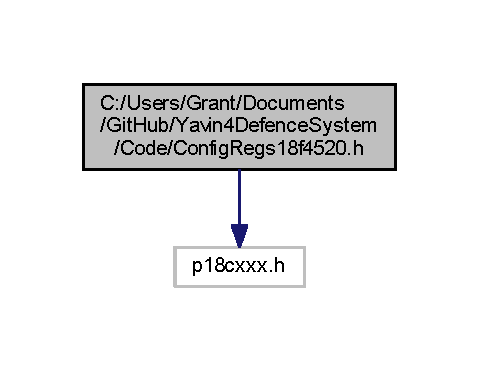
\includegraphics[width=188pt]{_config_regs18f4520_8h__incl}
\end{center}
\end{figure}


\subsection{Detailed Description}
Include file to set the Configuration Bits of a P\+I\+C18\+F4520. 

If the macro \+\_\+\+\_\+\+D\+E\+B\+U\+G is defined, the bits are set as appropriate for development and debugging\+:
\begin{DoxyItemize}
\item H\+S Oscillator; Oscillator Switch disabled; Power-\/\+On Timer;
\item Brown-\/out Reset disabled;
\item Watchdog Timer disabled;
\item C\+C\+P2 Multiplex disabled;
\item Stack Overflow Reset;
\item Low-\/voltage Programming disabled, Debug mode enabled;
\item No protection bits set.
\end{DoxyItemize}

If the macro \+\_\+\+\_\+\+D\+E\+B\+U\+G is N\+O\+T defined, the bits are set as appropriate for production code release\+:
\begin{DoxyItemize}
\item H\+S Oscillator; Oscillator Switch disabled; Power-\/\+On Timer;
\item Brown-\/out Reset enabled at 4.\+2\+V;
\item Watchdog Timer disabled;
\item C\+C\+P2 Multiplex disabled;
\item Stack Overflow Reset;
\item Low-\/voltage Programming and Debug mode disabled;
\item No protection bits set.
\end{DoxyItemize}

\begin{DoxyVersion}{Version}
0.\+1 -\/ derived from Config\+Regs18\+F452.\+h 
\end{DoxyVersion}
\begin{DoxyDate}{Date}
28-\/\+Aug-\/2014 
\end{DoxyDate}
\begin{DoxyAuthor}{Author}
David Rye
\end{DoxyAuthor}
\begin{DoxyNote}{Note}
This file was generated by the compiler from the command line\+: mcc18 -\/p18f4520 --help-\/config $>$ config\+Reg18\+F4520.\+h
\end{DoxyNote}
\begin{DoxyRefDesc}{Todo}
\item[\hyperlink{todo__todo000001}{Todo}]Consider if Watchdog Timer should be enabled for production code, and add W\+D\+T management code if so.\end{DoxyRefDesc}


\begin{DoxyRefDesc}{Todo}
\item[\hyperlink{todo__todo000002}{Todo}]Consider if Stack Overflow Reset should be enabled for production code. It may be better not to, as there is no re-\/entrant or recursive code, or dynamic memory allocation here -\/ if the code loads statically it should run.\end{DoxyRefDesc}


\begin{DoxyRefDesc}{Todo}
\item[\hyperlink{todo__todo000003}{Todo}]Change startup code c016iz.\+c so that everything (including initialised variables) correctly re-\/starts if \hyperlink{newmain_8c_acdef7a1fd863a6d3770c1268cb06add3}{main()} ever exits or a B\+O\+R or W\+D\+T reset occurs. \end{DoxyRefDesc}


Definition in file \hyperlink{_config_regs18f4520_8h_source}{Config\+Regs18f4520.\+h}.


%--- End generated contents ---

% Index
\newpage
\phantomsection
\addcontentsline{toc}{chapter}{Index}
\printindex

\end{document}
